\setlist{topsep=-2ex,itemsep=-2ex,partopsep=0ex,parsep=2ex}
\chapter{System Organization}
The new IDS architecture consists of three parts: memory transfer of packets from the CPU to the GPU, packet analysis on the GPU, and the transfer of inspection results back to the CPU.

\section{Memory Transfer of Packets to the GPU}
The CPU captures the packets using the APIs provided by the packet capture library LibPCAP ~\cite{bib4}. The packet capture library abstracts the packet capture process and provides a mechanism to capture packets from a live stream or to read packets from a saved file. These packets should be transferred from the CPU to the GPU. Due to the overhead associated with transferring data from the CPU to the GPU, all the packets are transferred into a buffer and the buffer is transferred to the GPU.

The system is divided into three components, packet capture, dissector and analysis as shown in Fig. ~\ref{fig:systemorganization}.

\begin{figure}[H]
	\centering
	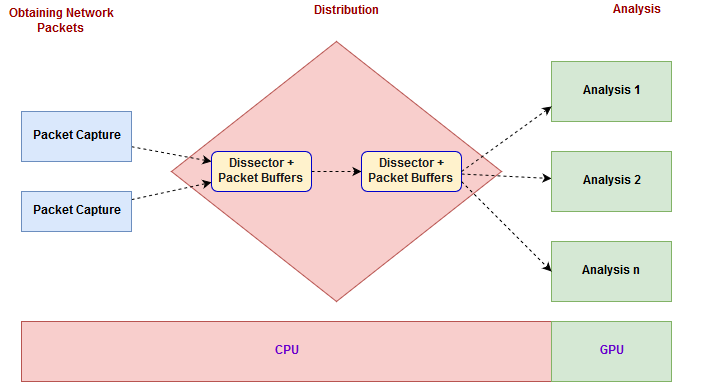
\includegraphics[width=14cm]{systemorganization.png}
	\caption[System organization]{System organization}
	\label{fig:systemorganization}
\end{figure}
\squeezeup

\begin{enumerate}[leftmargin=*]
	\item Packet Capture: This component captures the packets and saves them into packet buffers.
	\item Dissector: Dissector class consists of virtual functions, which are used to dissect the packet to obtain the attributes of the headers and the start of the payload.
	\item Analysis: This component works on the GPU and performs header checking and signature matching on the payload.
\end{enumerate}
\vspace{\topsep}

\section{Packet Capture Class}
The system defines PacketCapture as a class that is responsible for saving the packets into a PacketBuffer object. The PacketBuffer class has an array of packets that stores the raw data from the network and headers of the packets. The size of the packet buffer array is fixed and the kernel is launched with a specific number of threads that is divisible by the array size.
The PacketCapture class obtains the packets in two modes, live capture mode and off-line capture mode. 

\begin{enumerate}[leftmargin=*]
	\item Live capture mode: In this mode, the system can capture the packets in real-time and use them for surveillance and anomaly prevention.
	\item Off-line capture mode: In this mode, packets can be obtained from a TCP dump capture file or another source. They can be used to analyze and prevent a malicious attack in the future.
\end{enumerate}
\vspace{\topsep}

\section{Analysis}
The analysis is performed on the GPU using an array of packets that were transferred from the CPU. The analysis module is divided into three components, auto-mining, operations and hooks.
\begin{enumerate}[leftmargin=*]
	\item Auto-Mining: The entire packet analysis is distributed among the threads. As already mentioned, shared memory is much faster than global memory. Therefore, the data required for each thread are saved in shared memory in this module.
	\item Operations: In this module, the threads operate on the collected data. Header checking and signature matching are implemented. The naive, the Rabin-Karp, the Wu-Manber and the Aho-Corasick algorithms are used for signature matching. \\
	The results are written into an array after the rules are checked.
	\item Hooks: This module is written in C++. The results can be logged into a file, or a database, or they can be displayed on the console.
\end{enumerate}